%!TEX root = main.tex
\section{Introduction}
\subsection{Context}

The research described in the article is focus on providing the tool for estimating the run-time of a single CAL module (data processing program or algorithm). Computation Application Language (CAL) is designed to write large scale application in due to perform big data processing. Each CAL program consists of modules that are separetely executed in sequence (with parallelization possibility) on virtual machines and sending the results futher to a next module of the application. CAL language is a part of the system developed under the Baltic LSC\cite{baltic_lsc_website} project.

During the data processing within the application run, each module is executed with some input data. It could be different kind of data e.g. data frame or set of images. The execution of a module is invoke on a virtual machine with limited resources (RAM, mCPUs, GPUs). The properties of an input data and the execution environment resources will be used to estimate the overall application execution time and price on a specific cluster.

Baltic Large Scale Computing (BalticLSC\cite{baltic_lsc}) project is using CAL language to perform data processing tasks. Each task is an execution of a CAL application. Each module can be used in many CAL applications. We can say that a single module is a one block (commonly as a docker image) and an application is the schema of executing a sequence of blocks. Figure~\ref{fig:face_recogniser_app} shows the example application that consists of a few modules to perform a face recognition on the input video data. Some set of modules within a CAL application can be executed in parallel. Some modules can be also run as a multiple instances of itself to make data processing faster.

The worst-case complexity of an algorithm is the greatest number of operations needed to solve the problem over an input data of a given size. The analysis of algorithmic complexity emerged as a scientific subject during the 1960’s and has been quickly established as one of the most active fields of study\cite{complexity}. The most common way to describe an algorithm complexity is the \textit{big O} notation (collectively called Bachmann–Landau notation or asymptotic notation) which is the universal formula that describe how the run-time of an algorithm grow as the input data size grows. 

In our work, we study the formula (more precise and complex one in comparison to the \textit{big O} notation) that takes mixed sets of input data and run-time environment properties as arguments. Moreover, the models we introduce in further parts, will provide the estimation of the data processing program run-time and not only the complexity formula as it the \textit{big O} notation does. 

\begin{figure*}[!t]
	\centering
	\begin{minipage}{0.9\linewidth}
		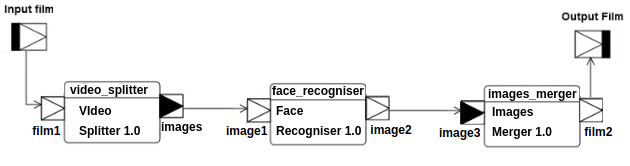
\includegraphics[width=1.0\textwidth]{face_recogniser_app}
	\end{minipage}
	\caption{\textit{Face Recogniser} scheme. Application written in the CAL language.}
	\label{fig:face_recogniser_app}
\end{figure*}

\subsection{Related work}

The articles listed above contain content that to some extent coincides with the research carried out in this article:

\begin{itemize}
	\item \textit{Estimation of the execution time in real-time systems}\cite{wcet} - an overview on the different approaches to estimate the program execution time. The authors focus on the \textit{WCET} concept. The aim for this project is not to estimate execution time as a deadline that could not be exceed. We try to estimate the average-case execution time (\textit{ACET}).

\item \textit{Execution Time Analysis for Embedded Real-Time Systems}\cite{time-analysis} - as is said in the section 5. of the article, a static timing  analysis tool works by statically analysing the properties of the program (embedded to a specific structure like vector or graph) that affect its timing behavior. Our approach, on the other hand, is to statically analyze the properties of input data and the run-time environment resources.

\item \textit{Using online worst-case execution time analysis and alternative tasks in real time systems}\cite{images-processing-time} - similar approach to carry out the regression using input data feature (section 3.6). The authors use an amount of image pixels as the only one feature to estimate the execution time of few different image processing algorithm.

\item \textit{A Prediction Model for Measurement-Based Timing Analysis}\cite{ga} - the authors made en experiment by generating random lists of data with the same properties and then train the artificial neural network to predict the \textit{WCET}. They used \textit{Gem5} to simulate the run-time environment. We have used the docker as an execution environment which allows to receive more real data with a natural noise introduce to the response variable (execution time). The authors develop their work in the next article\cite{surogate} using the concept of surogate models as a solution to the problem of generating training data. Such generating can increase overheads of the execution time estimation for processing algorithms with heavy input data.

\item \textit{Nonlinear approach for estimating WCET during programming phase}\cite{program-features} - the authors estimate a \textit{WCET} by extracting the program features from object code. It starts when the source code of a program is successfully compiled into object code. Then, the extracted features was used for subsequent samples optimization and \textit{WCET} estimate. The authors use SVR algorithm with RBF kelner as we did likewise.

\item \textit{A solution to minimum sample size for regressions}\cite{small-n} - the authors explore the problem of a small amount of training data which also affects the result of our article. Testing data generation and simple algorithm for the run-time estimation are used to reduce the impact of a small n problem on the final results of our work.

\end{itemize}

\subsection{Contribution}
Using simple machine learning algorithms (\textit{SVR} and \textit{KNN}, more about the algorithms and how they fit to the problem in the further sections) to estimate a program run-time. 

Determine the basic properties of an input data and run-time environment for data processing task. 

Creating a separate model for each module (program) instead of embedding the program structure to a vector of features or control flow graphs (CFGs).
